\section{Dataset}
\label{sec:dataset}

Our first contribution is the creation of a new open dataset which consists of images of dog poop in mostly
  urban, mostly outdoor environments, from mostly a single city.
The data is annotated to support object detection and segmentation tasks.
The majority of the images feature fresh poop from three specific medium sized dogs, but there are
  a significant number of images with poops of unknown age and from unknown dogs.

Despite these biases, the dataset has significant image variations.
To provide a gist, we computed UMAP \cite{mcinnes_umap_2020} image embeddings based on ResNet50
  \cite{he2016deep} descriptors display images corresponding with clusters in this embedding in
  \Cref{fig:umap_dataset_viz}.

More details about the dataset are available in a standardized datasheet
\cite{gebru_datasheets_2021} that covers the motivation, composition,
collection, preprocessing, uses, distribution, and maintenance. This will be
distributed with the data itself, and is provided in supplemental material.

\subsection{Dataset Collection}

A single researcher on dog walks photographed fresh dog poop, mostly their own
dogs, but often others. Distance was sometimes varied for diversity. Most
images were taken following the ``before/after/negative'' (BAN) protocol.  
A BAN triple comprises a ``before'' shot of the poop, an ``after'' shot
post removal, and a ``negative'' shot of a nearby lookalike (e.g., pine cones,
leaves).  We only use them for negative sampling, but they could enable
contrastive triplet losses \cite{schroff_facenet_2015}.

The majority of images follow the BAN protocol, but there are exceptions.
The first six months of data collection only involved the ``before/after'' part of the protocol. 
We began collecting the third negative image after a colleague suggested it.
In some cases, the researcher failed or was unable to take the second or third image.
These exceptions are often programmatically identifiable.
  
We also received 121 contributor images, mostly outside the BAN protocol.
These images are held out and used as our test set.
%These are used only for testing and are \emph{excluded} from the analysis in \Cref{subsec:datastat}.
Due to the small size, our main results also include validation scores.
%The small size of this test set is the reason that our main results include
%validation and test scores.

\subsection{Dataset Annotation}

Images were annotated using labelme \cite{wada_labelmeailabelme_nodate}.
Most annotations were initialized using SAM and a point prompt.
All AI polygons were manually reviewed.
In most cases only small manual adjustments were needed, but there were a significant number of cases where
  SAM did not work well and fully manual annotations were needed.
Regions with shadows seemed to cause SAM the most trouble, but there were other failure cases.
Unfortunately, there is no metadata to indicate which polygons were manually created or done using AI.
However, the number of vertices may be a reasonable proxy to estimate this, as polygons generated by SAM
  tend to have higher fidelity boundaries.
The boundaries of the annotated polygons are illustrated in \Cref{fig:compare_allannots}.

Data collected after 2024-07-03 was annotated with the help of models trained
on prior data. Again, all predictions were manually verified or corrected. In
these later cases, false positive annotations were labeled (e.g. stick, leaf),
but because these categories are not labeled exhaustively, we exclude them from
all analysis in this paper.


\begin{figure}[t]
\centering
\begin{subfigure}[t]{0.48\textwidth}
    \centering
    \includegraphics[width=\textwidth]{figures/images_timeofday_distribution.png}
    \caption{
        The time-of-year vs time-of-day of each image show lighting and seasonal
        variation.  On the x-axis, 0 is January 1st. On the y-axis, 0 is
        midnight.  Color estimates daylight based on location (if available).
        Most images are in the day, but many were taken at night with flash or
        long exposure.
    }
    \label{fig:TimeOfDayDistribution}
\end{subfigure}
\hfill
\begin{subfigure}[t]{0.48\textwidth}
    \centering
    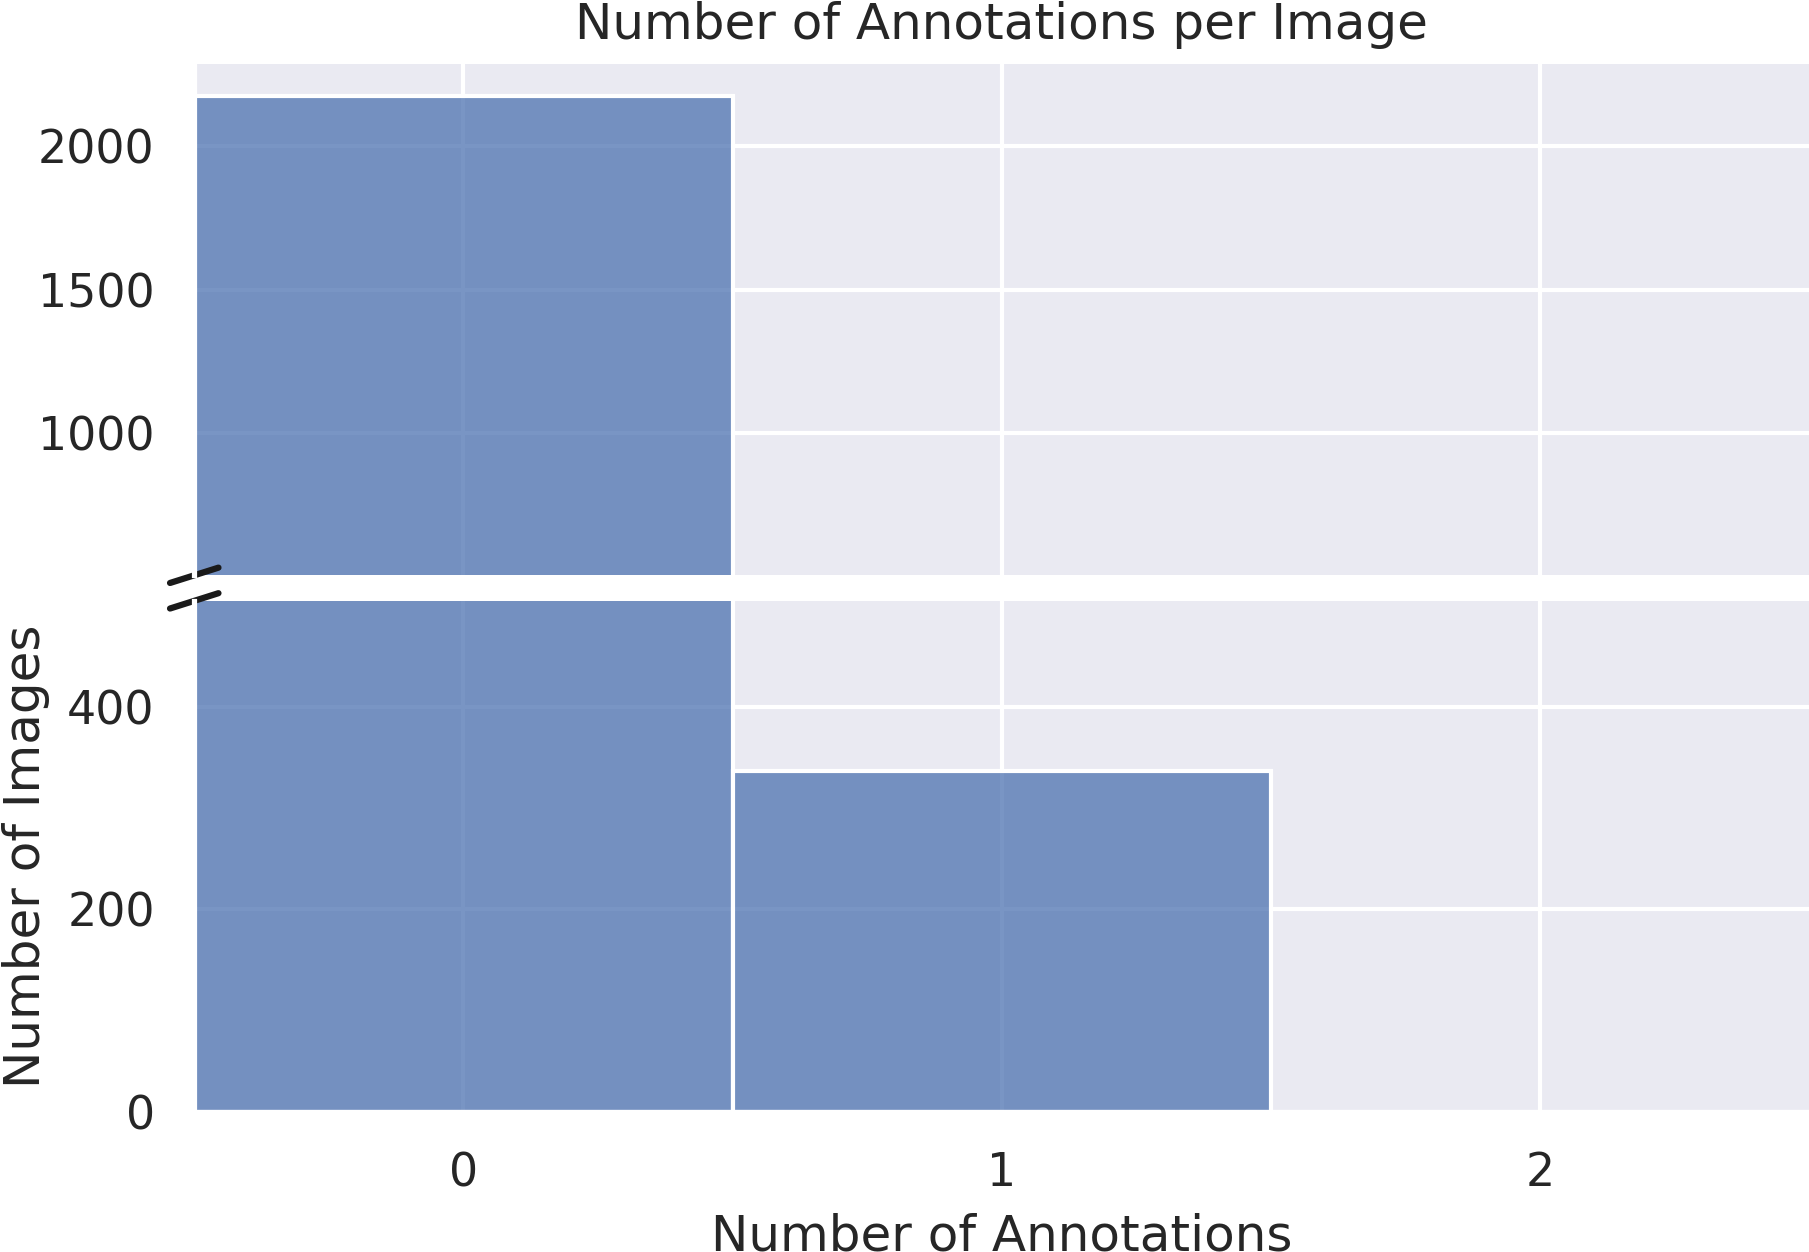
\includegraphics[width=\textwidth]{figures/anns_per_image_histogram_splity.png}
    \caption{
        The histogram of annotations per image shows object density variation.
        Only 35\% (3,314) of images contain annotations; 65\% (5,982) are known negatives.
        About half of the negatives were taken immediately after pickup; the
        rest are from nearby locations with potential lookalikes.
    }
    \label{fig:AnnotsPerImage}
\end{subfigure}
\caption{Dataset distributions. (a) Time and daylight scatterplot. (b) Annotation count histogram.}
\label{fig:TimeAndAnnots}
\end{figure}



\subsection{Dataset Properties and Statistics}
\label{subsec:datastat}

% Number of images, annotations, and other stats.

%import kwutil
%kwutil.datetime.coerce('now') - kwutil.datetime.coerce('2020-12-18')
%kwutil.datetime.coerce('2025-04-20') - kwutil.datetime.coerce('2020-12-18')

The data was captured at a regular rate over 4.3 years, primarily in parks and sidewalks within a small
  city.
Weather conditions varied across snowy, sunny, rainy, and foggy.
A visual representation of the distribution of seasons, time-of-day, daylight, and capture rate is provided
  in \Cref{fig:TimeOfDayDistribution}.

The dataset images are available in full resolution.
Almost all images were taken using the same phone-camera, with a consistent width/height of 4,032
  $\times$ 3,024 (although some may be rotated based on EXIF data).
The images are stored as 8-bit JPEGs with RGB channels, and most include overviews (i.e., image pyramids),
  allowing for fast loading of downscaled versions.
%Six images have a slightly different resolution of 4,008 $\times$ 5,344, and one has a resolution of 7,680
%  $\times$ 1,024.


Due to the BAN protocol, about one-third of the images contain
annotations, the rest were taken after the object(s) were removed.  Consequently, most
images have no annotations. When present, annotations are usually singular, but
multiple annotations are common and can be due to:
1) fragmented dropping,
2) dogs pooping together,
3) repeated poops in the same area over time (sometimes hard to distinguish from dirt).
The number of annotations per image is illustrated in \Cref{fig:AnnotsPerImage}.


\subsection{Dataset Splits}

Our dataset is split into training, validation, and test sets based on the year and day of image capture and
  photographer.
Only data captured by the authors is used for training and validation.
Of these, images from 2021-2023, 2025 and beyond are assigned to the training set. 
Images from 2020 are used for
  validation.
For data from 2024, we consider the ordinal date $n$ of each image and include it in the validation set if
  $n \equiv 0 \ (\textrm{mod}\ 3)$; otherwise, it is assigned to the training set.


For testing data, we use contributor images to not bias our results based on the way the authors took
  images.
These splits are provided in the COCO JSON format \cite{lin_microsoft_2014} as well as a WebDataset
  \cite{huggingfacewebdataset} on HuggingFace.
